\documentclass[11pt]{article}
\usepackage[margin=1in, top=0.3in]{geometry}
\usepackage[all]{nowidow}
\usepackage[hyperfigures=true, hidelinks, pdfhighlight=/N]{hyperref}
\usepackage[separate-uncertainty=true, group-digits=false]{siunitx}
\usepackage{graphicx,amsmath,physics,tabto,float,amssymb,pgfplots,verbatim,tcolorbox}
\usepackage{listings,xcolor,subfig,caption,import,wrapfig}
\usepackage[version=4]{mhchem}
\numberwithin{equation}{section}
\numberwithin{figure}{section}
\numberwithin{table}{section}
\definecolor{stringcolor}{HTML}{C792EA}
\definecolor{codeblue}{HTML}{2162DB}
\definecolor{commentcolor}{HTML}{4A6E46}
\captionsetup{font=small, belowskip=0pt}
\lstdefinestyle{appendix}{
    basicstyle=\ttfamily\footnotesize,commentstyle=\color{commentcolor},keywordstyle=\color{codeblue},
    stringstyle=\color{stringcolor},showstringspaces=false,numbers=left,upquote=true,captionpos=t,
    abovecaptionskip=12pt,belowcaptionskip=12pt,language=Python,breaklines=true,frame=single}
\lstdefinestyle{inline}{
    basicstyle=\ttfamily\footnotesize,commentstyle=\color{commentcolor},keywordstyle=\color{codeblue},
    stringstyle=\color{stringcolor},showstringspaces=false,numbers=left,upquote=true,frame=tb,
    captionpos=b,language=Python}
\renewcommand{\lstlistingname}{Appendix}
\pgfplotsset{compat=1.17}

\begin{document}

\begin{center}
    {\huge Determining the Rydberg constant from the Balmer series of hydrogen}\\
    \vspace{0.2in}
    \textbf{KDSMIL001 | 18 August 2021}
    
    
    \section*{Abstract}\label{sec:Abstract}
    We found a value for the Rydberg constant by measuring the wavelengths of the visible hydrogen emission spectral lines and using the Rydberg formula for the Balmer series to fit those wavelengths to a linear plot. We found our value to not agree with the literature value and suspect that is a result of the way we calibrated our equipment.
\end{center}
    
\section{Introduction}\label{sec:Introduction}
\par The Balmer series is a describes a subset of the spectral line emissions of a hydrogen atom. The wavelengths of the lines in this series are given by the formula
\begin{equation}
    \frac{1}{\lambda}=R\left(\frac{1}{n^2}-\frac{1}{m^2}\right)\cite{Foot}
    \label{eqn:Balmer}
\end{equation}
where $n=2$, $m=3,4,5,\dots$, and $R$ is the Rydberg constant, given by
\begin{equation}
    R=\frac{m_ee^4}{8\varepsilon^2h^3c}=\SI{10973731.568160(21)}{\metre^-1}\cite{CODATA}
    \label{eqn:Rydberg Constant}
\end{equation}
\par Note that \autoref{eqn:Balmer} describes much more than just the Balmer series but only the Balmer series is needed for this experiment, and only 4 of the many spectral lines in the series at that. These 4 lines are called H-$\alpha$ (m=3), H-$\beta$ (m=4), H-$\gamma$ (m=5), and H-$\delta$ (m=6) and they will be used as they are the 4 that (formally) lie within the visible spectrum.
\par To determine a value for $R$, the wavelengths of H-$\alpha$, H-$\beta$, H-$\gamma$, and H-$\delta$ will be measured and a linear fit will be made with $\left(\frac{1}{2^2}-\frac{1}{m^2}\right)$ as the x values and $\frac{1}{\lambda}$ as the y values, thus $R$ will be the gradient.

\section{Apparatus}\label{sec:Apparatus}
\par A Heath EU-700 Czerny-Turner monochromator with a photo-multiplier detector and pulse-counting electronics was used to measure the wavelengths of the spectral lines coming from a hydrogen spectral tube. The measurement system has three primary measurement parameters: slit width, dwell time, and step increment. The system counts how many times a photon was incident on the detector for the given wavelength, incrementing through a range of wavelengths measured in Angstroms.
\par The monochromator reports an incorrect wavelength, off by about 20 Angstroms, so the set-up needed to be calibrated. A HeNe laser of known wavelength (6328 A) was fired at the measurement system as show in \autoref{fig:Calibration Set-up}.

\begin{figure}[H]
    \begin{center}
        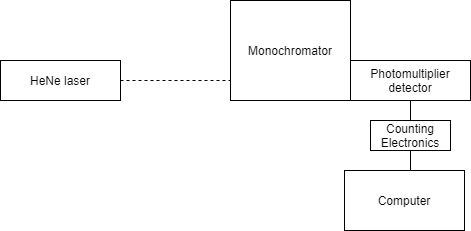
\includegraphics[width=.65\textwidth]{calibration.png}
        \caption{Calibration set-up}
        \label{fig:Calibration Set-up}
    \end{center}
\end{figure}

\section{Method}\label{sec:Method}
\subsection{Calibration}\label{sec:Calibration}
\par Using the wavelength of the HeNe laser (6328 A) as a known value, measurements were made with a variety of parameters, the details of which can be found in \autoref{sec:Calibration Data}, around the expected value. Gaussians could be fitted to the data using \texttt{scipy.optimize.curve\_fit} and a $\mu$ and $\sigma$ extracted for each set. The difference between this $\mu$ and the known wavelength is the correction factor that needs to be applied to all measurements taken with this set-up. These corrections were combined in a mean weighted by their uncertainty $\sigma$ using
\begin{align}
    \bar \mu_{wtd}&=\frac{\sum\limits_{i=1}^nw_i\mu_i}{\sum\limits_{i=1}^nw_i}\label{eqn:Weighted Mean}\\
    \sigma_{wtd}&=\sqrt{\frac{\frac{\sum\limits_{i=1}^nw_i\mu_i^2}{\sum\limits_{i=1}^nw_i}-(\bar\mu_{wtd})^2}{n-1}}\label{eqn:Weighted Mean Uncertainty}
\end{align}
where $w_i=\frac{1}{\sigma^2}$ is the weighting \cite{Data Reduction}. 
\par The count data was assumed to be Poissonian and thus the uncertainty on a count of $N$ is simply $\sqrt{N}$. This uncertainty was provided to \texttt{curve\_fit}. \autoref{fig:Calibration Main} shows an example of one calibration run. The final correction was found to be \num{-22.46\pm0.14}.

\begin{figure}[h]
    \begin{center}
       \scalebox{0.75}{\subimport{Plots}{calibrationMain.pgf}}
       \caption{Calibration data with slit width $\SI{10}{\mu\m}$, dwell time $\SI{200}{m\second}$, increment 0.5 A, and on the range 6300-6400 A. The Gaussian was fit using \texttt{scipy.optimize.curve\_fit} with the initial guess $\mu=$ the position of the maximum of the data and $\sigma=1$. A vertical shift was included to account for background and an amplitude to account for Gaussians being a PDF.}
       \label{fig:Calibration Main}
    \end{center}
\end{figure}

\subsection{Data}\label{sec:Data}
\par Mesurements were made for each of the spectral lines with a variety of parameters, the details of which can be found in \autoref{sec:Spectral Line Data}, and their wavelengths found as in \autoref{sec:Calibration} by fitting a Gaussian. After subtracting the correction factor and combining the uncertainties of the wavelength and correction factor in quadrature, the wavelengths found for each spectral line were combined using \autoref{eqn:Weighted Mean} and \autoref{eqn:Weighted Mean Uncertainty} where again $w_i=\frac{1}{\sigma^2}$. \autoref{fig:DataMain} shows an example for the fitting done.

\begin{figure}[H]
    \begin{center}
       \scalebox{0.75}{\subimport{Plots}{dataMain.pgf}}
       \caption{Data for spectral line H-$\delta$ with slit width $\SI{100}{\mu\m}$, dwell time $\SI{300}{m\second}$, increment 0.2 A, and on the range 4099-4150 A. The expected wavelength is \num{4101.734\pm0.006}\cite{Spectral Lines} and after correction the measured wavelength is \num{4100.0\pm1.1}. The initial conditions for this fit were as in \autoref{fig:Calibration Main}}
       \label{fig:DataMain}
    \end{center}
\end{figure}

\par After wavelengths $\lambda$ were found for each spectral line, a weighted linear least squares fit was performed as described in \cite{Kirkup} with the x values being $\left(\frac{1}{2^2}-\frac{1}{m^2}\right)$ and the y values being $1/\lambda$. Uncertainties on the y values were $\frac{u(\lambda)}{\lambda^2}$. The gradient of this linear fit gives a value for $R$.

\section{Results}\label{sec:Results}
\begin{table}[H]
    \centering
    \begin{tabular}{c|c|c}
         & Measured & Literature \\\hline
        H-$\alpha$ & \SI{6563.013\pm0.041}{A} & \SI{6562.79\pm0.03}{A} \\\hline
        H-$\beta$ & \SI{4859.94\pm0.66}{A} & \SI{4861.35\pm0.05}{A}\\\hline
        H-$\gamma$ & \SI{4338.945\pm0.043}{A} & \SI{4340.472\pm0.006}{A}\\\hline
        H-$\delta$ & \SI{4100.006\pm0.053}{A} & \SI{4101.734\pm0.006 }{A}
    \end{tabular}
    \caption{The measured and literature values for the wavelengths of the spectral lines for the Balmer series in hydrogen, measured in Angstrom. Literature values found in \cite{Spectral Lines}. Note the large uncertainty for H-$\beta$ as there were fewer runs available for that wavelength.}
    \label{tbl:Spectral Lines}
\end{table}

\begin{figure}[H]
    \begin{center}
       \scalebox{0.75}{\subimport{Plots}{fit.pgf}}
       \caption{Weighted linear least squares fit of the inverse of the measured spectral line wavelengths to \autoref{eqn:Balmer}. The uncertainty on the inverse wavelengths is plotted but due to the method described in \autoref{eqn:Rydberg Constant} and \autoref{eqn:Weighted Mean Uncertainty}, these uncertainties are reduced to the point of being unnoticeable at this scale. The slope $m$ is the Rydberg constant $R$.}
       \label{fig:Fit}
    \end{center}
\end{figure}

\section{Discussion and Recommendations}\label{sec:DiscussionRecommendations}
\par We find the Rydberg constant to be $\SI{10983450\pm280}{\metre^-1}$, which does not agree within experimental uncertainty with the literature value of $\SI{10973731.568160(21)}{\metre^-1}$\cite{CODATA}. Note that when discussing hydrogen specifically, the Rydberg constant is modified to account for the small mass of the element: $R_H=R\frac{m_p}{m_e+m_p}\cite{Foot}=\SI{10967758.340\pm0.0033}{\metre^-1}$, where $m_e$ is the reduced mass of the electron and $m_p$ is the mass of the proton \cite{CODATA}. We see that our measured value is even further from $R_H$ than from $R$. 
\par In the interest of a sanity check, we performed the same linear fitting using the literature values for the wavelengths of the four spectral lines, found in \cite{Spectral Lines}, and found a value of $R=\SI{10971003\pm93}{\metre^-1}$, which still does not agree with $R_H$, but is at least closer to it than our value, implying that our technique is valid to some extent, but our data is where the problem lies.
\par As can be seen in \autoref{tbl:Spectral Lines}, the uncertainty on our wavelengths, aside from H-$\beta$ which did not have the same amount of data, are all approximately the same, and yet the difference between our value and the literature value varies considerably from line to line. This leads us to believe that the main reason for the discrepancy in measured values for $R$ is that the calibration we performed was not sufficient. We suspect that the relationship between measured wavelength and actual wavelength is not linear, or at least was not accurately captured by our one data point. We recommend calibrating using more than one laser, or capturing more than one known wavelength in some other way.

\section{Conclusion}\label{sec:Conclusion}
\par We found the value of the Rydberg constant to be $\SI{10983450\pm280}{\metre^-1}$, which does not agree with the literature value of either $R$ or $R_H$ within experimental uncertainty. We suspect that this is a result of the insufficient calibration method and recommend using more than one known wavelength to calibrate. Another source of uncertainty could lie in our lack of good data for the H-$\beta$ spectral line and we recommend using more than one dataset per wavelength.


\begin{thebibliography}{9}
    \bibitem{CODATA}
    2018 CODATA list of the Fundamental Physical Constants, \texttt{https://physics.nist.gov/cuu/Constants/Table/allascii.txt}
    \bibitem{Foot}
    Foot, C., \textit{Atomic Physics}, Oxford University Press, 2005
    \bibitem{Data Reduction}
    Bevington, P. R., \textit{Data Reduction and Error Analysis for the Physical Sciences}, McGraw-Hill, 1969
    \bibitem{Spectral Lines}
    Kramida, A., Ralchenko, Yu., Reader, J., and NIST ASD Team (2020). NIST Atomic Spectra Database (ver. 5.8), [Online]. Available: \texttt{https://physics.nist.gov/asd} [2021, August 21]. National Institute of Standards and Technology, Gaithersburg, MD. DOI: \texttt{https://doi.org/10.18434/T4W}
    \bibitem{Kirkup}
    Kirkup, L., \textit{Experimental methods for science and engineering students}, (2019)
\end{thebibliography}


\newpage
\section{Appendix}\label{sec:Appendix}
\setcounter{figure}{0} \renewcommand{\thefigure}{A.\arabic{figure}}
\subsection{Calibration Data}\label{sec:Calibration Data}


\subsection{Spectral Line Data}\label{sec:Spectral Line Data}

\end{document}
